\documentclass{article}
\usepackage{tikz}
\usepackage{amsmath}
%
\begin{document}
%
% paper title
\title{ANN}
\author{Craig~Euler}
%
\maketitle
%
\begin{center}
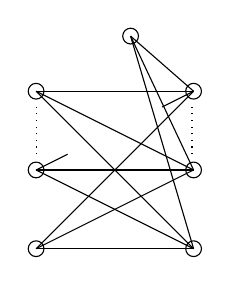
\begin{tikzpicture}
\draw (0.0, 0.0) circle (0.1cm);
\draw (0.0, 1.0) circle (0.1cm);
\draw (0.0, 2.0) circle (0.1cm);

\draw (2.0, 2.0) circle (0.1cm);
\draw (2.0, 0.0) circle (0.1cm);
\draw (2.0, 1.0) circle (0.1cm);
\draw (1.2, 2.7) circle (0.1cm);

\draw (0.0, 0.0) -- (2.0, 0.0);
\draw (0.0, 0.0) -- (2.0, 1.0);
\draw (0.0, 0.0) -- (2.0, 2.0);

\draw (0.0, 1.0) -- (2.0, 0.0);
\draw (0.0, 1.0) -- (2.0, 1.0);
\draw (0.0, 1.0) -- (0.4, 1.2);
\draw (1.6, 1.8) -- (2.0, 2.0);

\draw (0.0, 2.0) -- (2.0, 0.0);
\draw (0.0, 2.0) -- (2.0, 1.0);
\draw (0.0, 2.0) -- (2.0, 2.0);

\draw (1.2, 2.7) -- (2.0, 0.0);
\draw (1.2, 2.7) -- (2.0, 1.0);
\draw (1.2, 2.7) -- (2.0, 2.0);
\draw[dotted] (0.01, 1.2) -- (0.01, 1.8);
\draw[dotted] (1.98, 1.2) -- (1.98, 1.8);
\end{tikzpicture}
\end{center}
%
Back propagation derivation for the ANN.

A caveat: the range for summation indexing is assumed from context in these notes.

First define some shorthand:
\begin{equation} \label{eq:psi}
\psi^i_p = \sum_{k} y_k^i \omega_{p,k}^i + b^iu_p^i
\end{equation}
%
The first, interior, and last layers are denoted with $x$, $y$, and $z$ respectively. Hence, \eqref{eq:psi} will differ with the respective layer.
%
\begin{equation} \label{eq:z}
z_p := g(\psi_p^N)
\end{equation}
%
where $g$ is the activation function typically defined as:
%
\begin{equation} \label{eq:g}
g(x;\beta) := \frac{1}{1 + e^{-\beta x}}
\end{equation}
%
and so it follows that the derivative of the activation function would be
%
\begin{equation} \label{eq:gp}
g'(x;\beta) = \beta \left( 1 - g(x;\beta) \right) g(x; \beta).
\end{equation}
%
\begin{equation} \label{eq:z}
y_p^{i+1} := g(\psi_p^i)
\end{equation}
%
\begin{equation} \label{eq:error}
E := \frac{1}{2} \sum_k (z_k - t_k)^2
\end{equation}
%
then
%
\begin{equation} \label{eq:derror}
\frac{\partial E}{\partial z_p} = z_p - t_p
\end{equation}
%
at the last layer:
%
\begin{equation} \label{eq:last_layer_derror}
\frac{\partial E}{\partial \omega_{i,j}^N} =
\left[ \frac{\partial E}{\partial z_i} \right] \left[ \frac{\partial z_i}{\partial \omega_{i, j}^N} \right] =
\left[ z_i - t_i \right] \left[ y_j^N g' (\psi_i^N) \right] =
\frac{\partial E}{\partial \omega_{i,j}^N}
\end{equation}
%
notice that
%
\begin{equation} \label{eq:last_layer_derror_eq_0}
\frac{\delta z_i}{\delta \omega_{p,j}} = 0
\end{equation}
%
$\forall i \neq p$. Defining
%
\begin{equation} \label{eq:delta}
\delta_{i,j}^N := \frac{\partial E}{\partial \omega_{i,j}^N}
\end{equation}
%
expanding \eqref{eq:delta} with \eqref{eq:last_layer_derror}:
%
\begin{equation} \label{eq:delta_full}
\delta_{i,j}^n = 
\left ( z_i - t_i \right ) y_j^n g' (\psi_i^n)
\end{equation}
%
\begin{equation} \label{eq:gamma}
\gamma_{i,j} := (z_j - t_j) g'(\psi_j^N)
\end{equation}
%
or, equivalently,
%
\begin{equation} \label{eq:gamma_array}
\gamma_i := \sum_j (z_j - t_j) g'(\psi_j^n)
\end{equation}
%
then
%
\begin{equation} \label{eq:delta2}
\delta_{i,j}^{n-1} =
\sum_{k_{n+1}} \delta_{k_{n+1},j}^n \omega_{k_{n+1},i}^n
\end{equation}
%
and
%
\begin{equation} \label{eq:end_weights}
\omega_{new}^N = \omega_{old}^N - \eta \delta^N
\end{equation}
%
interior weights, for $p < N$, are updated as follows:
%
\begin{equation} \label{eq:w_weights}
\omega_{new}^p = \omega_{old}^p - \eta \delta_w^p
\end{equation}
%
\begin{equation} \label{eq:u_weights}
u_{new}^p = u_{old}^p - \eta \delta_u^p
\end{equation}
%
where
%
\begin{equation} \label{eq:w_delta}
\delta_w^{q} = g'(\psi^{q}) (y^{q})^T \odot (\omega^{q+1})^T (\zeta^{q+2})^T ... (\zeta^N)^T (\gamma)^T
\end{equation}
%
\begin{equation} \label{eq:u_delta}
\delta_u^{q} = g'(\psi^{q}) (b^{q})^T \odot (\omega^{q+1})^T (\zeta ^{q+2})^T ... (\zeta^N)^T (\gamma)^T
\end{equation}
%
where
%
\begin{equation} \label{eq:u_delta}
\zeta_{i,j}^q = \omega_{i,j}^q y_j^{\prime q} = \omega_{i,j}^q \beta (1 - y_j^q) y_j^q
\end{equation}
%
\end{document}
